\chapter{Equiangular lines and the second eigenvalue multiplicity}

We are now going to discuss a geometric application of spectral graph theory.
A set of lines passing through the origin in $\R^d$ is called \textit{equiangular} if the angle between any two distinct lines is the same.
How large can such a set be in a fixed dimension $d$?
If $d = 2$, the best construction consists of three lines with pairwise angle $\pi /3$ (see Figure \ref{fig:equiangular-lines}).

\begin{figure}[ht]
    \centering
    \begin{tikzpicture}
        \coordinate (m) at (0:0);
    
        \foreach \i in {1, 2, ..., 6} {
            \coordinate (v\i) at ({360/6 * (\i - 1) + 90} : 1.5);
        }

        \pic [thick, draw=red!50, fill=red!20, ->, angle eccentricity = 1.5, "\footnotesize $\pi / 3$", pic text options={shift={(5pt,0)}}] 
            {angle = v5--m--v6};

        \draw[thick] (v1) -- (v4);
        \draw[thick] (v2) -- (v5);
        \draw[thick] (v3) -- (v6);
    \end{tikzpicture}
    \captionsetup{justification=centering, margin=2cm}
    \caption{Equiangular lines in two dimensions}
    \label{fig:equiangular-lines}
\end{figure}

Even though it may seem utterly unrelated to graph theory at first sight, the problem of determining the maximum number of equiangular lines $N(d)$ in a given dimension $d$ is considered one of the founding problems of spectral graph theory (see \mbox{\cite[Chapter 11]{godsilroyle})}.

Besides that, a slightly different problem has been studied, where the common angle between the lines is held fixed and the dimension $d$ tends to infinity.
For $\alpha \in (0, 1)$, let $N_\alpha (d)$ denote the maximum number of equiangular lines in $\R^d$ with pairwise angle $\arccos \alpha$.
In a remarkable work, Jiang, Tidor, Yao, Zhang, and Zhao recently determined $N_\alpha (d)$ for all sufficiently large dimensions $d$ using techniques of spectral graph theory. 
The discussion of their paper \cite{equiangular} will be the focus of this chapter.

\section{Graphs and equiangular lines}
Clearly, any line passing through the origin can be represented by a unit vector in the same direction. 
Hence, a set of $k$ equiangular lines corresponds to a set $S = \{ \bm{x}_1, \dots, \bm{x}_k \}$ of unit vectors in $\R^d$. 
This set is not unique: Any of the vectors $\bm{x}_i$ can be replaced by $-\bm{x}_i$, which spans the same line.
If $S$ is such a set of unit vectors representing a set of equiangular lines with pairwise common angle $\arccos \alpha$, $\alpha \in (0, 1)$, we have 
\begin{equation*}
    \bm{x}_i^T \bm{x}_j = \pm \alpha
\end{equation*}
for all $i \ne j$. 
We now define an associated graph $G$ with vertex set $S$ and an edge between $\bm{x}_i$ and $\bm{x}_j$ whenever $\bm{x}_i^T \bm{x}_j = -\alpha$, i.e. whenever the two vectors form an obtuse angle.
Consider the Gram matrix $M$ of the vectors in $S$ with entries $M_{ij} = \bm{x}_i^T \bm{x}_j$.
The matrix $M$ has rank at most $d$, is positive semidefinite (see \cite[Theorem 7.2.10]{matrixanalysis}) and is of the form
\begin{equation*}
    M = (1- \alpha)I + \alpha (J - 2 A_G),
\end{equation*}
where $A_G$ denotes the adjacency matrix of the associated graph defined above.

Conversely, given any graph $G$ and $\alpha \in (0,1)$, we can define the matrix
\begin{equation*}
    M_G = (1- \alpha)I + \alpha (J - 2 A_G).
\end{equation*}
If this matrix has rank $d$ and is positive semidefinite, it is the Gram matrix of a set of vectors in $\R^d$, which must have mutual inner product $\pm \alpha$, and hence correspond to a set of equiangular lines in $\R^d$.

Therefore, the problem of finding equiangular lines in $\R^d$ has an equivalent graph-theoretic formulation:
\begin{lemma} \label{lem:equiangularlines-equivalent-condition}
    Let $\alpha \in (0, 1)$. There exists a family of $N$ equiangular lines in $\R^d$ with common angle $\arccos \alpha$ if and only if there is an $N$-vertex graph $G$ such that the matrix 
    \begin{equation*}
        M_G = (1- \alpha)I + \alpha (J - 2 A_G)
    \end{equation*}
    has rank at most $d$ and is positive semidefinite.
\end{lemma}

\begin{remark}
    Clearly, $M_G$ has rank at most $d$ and is positive semidefinite if and only if the same holds for the matrix divided by $2\alpha$.
    Hence, letting $\lambda = (1 - \alpha)/(2 \alpha)$, it is equivalent to consider the matrix
    \begin{equation*}
        \lambda I - A_G + \frac{1}{2} J.
    \end{equation*}
\end{remark}

Using the reduction above, Lemmens and Seidel \cite{lemmensseidel} published the following general upper bound on the number of equiangular lines in a given dimension:
\begin{theorem}
    For every $d \in \N$, the maximum number $N(d)$ of equiangular lines in $d$ dimensions satisfies $N(d) \le \frac{1}{2} d (d + 1)$.
\end{theorem}
Moreover, de Caen \cite{decaen} gave a construction of $\frac{2}{9} (d + 1)^2$ equiangular lines in $d$ dimensions, when $d$ is of the form $d = 3 \cdot 2^{2 t - 1} - 1$ with $t \in \N$.
His result in particular implies that $N(d) = \Theta (d^2)$ for all $d$.

Now let $\alpha \in (0, 1)$ be fixed. 
Recall that the maximum number of equiangular lines in $\R^d$ with pairwise common angle $\arccos \alpha$ is denoted by $N_\alpha (d)$.
As it turns out, this quantity shows quite a different behaviour than $N(d)$: 
Bukh \cite{bukh} proved that $N_\alpha(d)$ grows only linearly in $d$ for any fixed $\alpha$, in contrast to $N(d) = \Theta(d^2)$.
However, the precise value of $\limsup_{d \rightarrow \infty} N_\alpha (d) / d$ remained open for arbitrary $\alpha$ until the recent work of Jiang, Tidor, Yao, Zhang, and Zhao \cite{equiangular}.

In order to state their results, we need the following graph-theoretic quantity.
\begin{definition}
    Let $\lambda > 0$. 
    The \textit{spectral radius order} $k = k(\lambda)$ of $\lambda$ is the smallest integer such that there exists a graph $G$  on $k$ vertices with spectral radius $\lambda_1(G) = \lambda$. 
    If no such graph exists, then $k(\lambda) = \infty$.
\end{definition}

The following is the main result from \cite{equiangular}.
In addition to determining \sloppy $\lim_{d \rightarrow \infty} N_\alpha(d) / d$ for all $\alpha$, they also exhibit the exact value of $N_\alpha(d)$ for those $\alpha$ where the limit is greater than 1, and $d$ is large enough.

\begin{theorem}[{\cite[Theorem 1.2]{equiangular}}] \label{thm:equiangular-lines}
    Fix $\alpha \in (0, 1)$. 
    Let $\lambda = \frac{1 - \alpha}{2 \alpha}$ and let $k = k(\lambda)$ be its spectral radius order. 
    \begin{enumerate}
        \item If $k < \infty$, there exists $d_0 (\alpha) \in \N$ such that
            \begin{equation*}
                N_\alpha (d) = \left \lfloor \frac{k (d - 1)}{k - 1}  \right \rfloor
            \end{equation*}
            for all dimensions $d \ge d_0 (\alpha)$.
        \item If $k = \infty$, then $N_\alpha (d) = d + o(d)$ as $d \rightarrow \infty$.
    \end{enumerate}
\end{theorem}

If $\alpha$ is one over an odd integer, then the result can be expressed in a simpler form. 
\begin{corollary}
    Let $k \ge 2$ be an integer and $\alpha = 1 / (2k - 1)$. Then, for all sufficiently large $d$, one has
    \begin{equation*}
        N_\alpha(d) = \left \lfloor \frac{k (d - 1)}{k - 1}  \right \rfloor.
    \end{equation*}
\end{corollary}

\begin{proof}
    We have 
    \begin{equation*}
        \lambda = \frac{1 - \alpha}{2 \alpha} = \frac{1 - \frac{1}{2k - 1}}{\frac{2}{2k - 1}} = \frac{2k - 2}{2k - 1} \cdot \frac{2k - 1}{2} = k - 1,
    \end{equation*}
    and the complete graph $K_{k}$ is the smallest graph with spectral radius $k - 1$. 
\end{proof}

A key ingredient in the proof of Theorem \ref{thm:equiangular-lines} is that graphs with bounded maximum degree have sublinear second eigenvalue multiplicity.

\begin{theorem}[{\cite[Theorem 2.2]{equiangular}}] \label{thm:snd-eigval-multiplicity}
    Let $\Delta > 0$. 
    For every connected graph on $n$ vertices with maximum degree at most $\Delta$, the multiplicity of the second-largest eigenvalue is at most $O_\Delta (n / \log \log n)$
    \footnote{The notation $O_\Delta (\dots)$ means that the implied constant may depend on $\Delta$.}
    \mbox{.}
\end{theorem}

While there are many classical results about the magnitude of the second-largest eigenvalue, remarkably little is known about eigenvalue multiplicities in general graphs.
To the best of our knowledge, the above theorem is the first result to provide a sublinear bound for any general graph class.
Due to the importance of the second eigenvalue, it can be considered a significant advance in spectral graph theory in its own right.
The proof of the theorem will be discussed in Section \ref{section:snd-eigval-multiplicity}.

We aim to apply Theorem \ref{thm:snd-eigval-multiplicity} to the graph associated with a set of equiangular lines. 
The following result tells us that we can choose a set of unit vectors such that the associated graph has bounded maximum degree.

\begin{theorem}[{\cite[Theorem 2.1]{equiangular}}] \label{thm:bounded-degree-associated-graph}
    For every $\alpha \in (0, 1)$, there exists a constant $\Delta = \Delta(\alpha)$ such that the following holds. 
    For every set of equiangular lines in $\R^d$ with pairwise common angle $\arccos \alpha$, one can choose a set $S$ of unit vectors in $\R^d$ representing the equiangular set such that each vector in $S$ has inner product $-\alpha$ with at most $\Delta$ other vectors in $S$.
\end{theorem}

We will prove this theorem in Section \ref{section:bounded-degree-graph}.

\section{Proof of the equiangular lines theorem}
In this section, we prove Theorem \ref{thm:equiangular-lines}, assuming that Theorems \ref{thm:snd-eigval-multiplicity} and \ref{thm:bounded-degree-associated-graph} hold.
The lower and upper bounds of the theorem are restated separately as Propositions \ref{prop:equiangular-lines-lower-bounds} and \ref{prop:equiangular-lines-upper-bounds} below.
Throughout the section, let $\alpha \in (0, 1)$ be fixed and $\lambda = (1 - \alpha) / (2 \alpha)$.

\begin{proposition}[Lower bounds] \label{prop:equiangular-lines-lower-bounds}
    For any $d \in \N$, we have $N_\alpha(d) \ge d$. 
    If \mbox{$k = k(\lambda) < \infty$}, then $N_\alpha(d) \ge \lfloor k(d- 1) / (k - 1) \rfloor$.
\end{proposition}

\begin{proof}
    First observe that $J_n$ is positive semidefinite, since its eigenvalues (namely $n$ and $0^{(n - 1)}$) are all nonnegative.
    Furthermore, recall that a positive linear combination of positive semidefinite matrices is also positive semidefinite.
    
    We start by showing $N_\alpha(d) \ge d$.
    Let $G$ be the empty graph on $d$ vertices, such that $A_G = 0$, and the associated matrix is $\lambda I_d + \frac{1}{2}J_d$.
    This matrix has rank $d$ and is positive semidefinite since it is a positive linear combination of $I$ and $J$, both of which are positive semidefinite.
    Hence, by Lemma \ref{lem:equiangularlines-equivalent-condition}, we have $N_\alpha(d) \ge d$.

    Now assume $k = k(\lambda) < \infty$, and consider a graph $H$ on $k$ vertices with spectral radius $\lambda_1(H) = \lambda$.
    Note that $H$ must be connected since $k$ is the smallest possible number of vertices of such a graph. 
    By the Perron--Frobenius theorem, it follows that the multiplicity of $\lambda$ in $H$ is $1$.
    Let $G$ be the disjoint union of $\lfloor (d - 1) / (k - 1) \rfloor$ copies of $H$ together with $(d - 1) - (k - 1) \lfloor (d - 1) / (k - 1) \rfloor$ isolated vertices.
    The graph $G$ has 
    \begin{equation*}
        k \left \lfloor \frac{d - 1}{k - 1} \right \rfloor + (d - 1) - (k - 1) \left \lfloor \frac{d - 1}{k - 1} \right \rfloor 
            = d - 1 + \left \lfloor \frac{d - 1}{k - 1} \right \rfloor 
            = \left \lfloor \frac{k (d- 1)}{k - 1} \right \rfloor
    \end{equation*}
    vertices, and top eigenvalue $\lambda$ with multiplicity $\lfloor (d - 1) / (k - 1) \rfloor$.
    It remains to show that $\lambda I - A_G + \frac{1}{2} J$ has rank at most $d$ and is positive semidefinite.
    Since the eigenvalues of $A_G$ are not larger than $\lambda$, the eigenvalues of $\lambda I - A_G$ are all nonnegative and hence the matrix is positive semidefinite.
    As for the rank, $\lambda I - A_G$ has the eigenvalue $0$ with multiplicity $\lfloor (d - 1) / (k - 1) \rfloor$, and therefore 
    \begin{equation*}
        \rank (\lambda I - A_G) = \left \lfloor \frac{k (d- 1)}{k - 1} \right \rfloor - \left \lfloor \frac {d - 1}{k - 1} \right \rfloor = d - 1.
    \end{equation*}
    Since $\frac{1}{2} J$ has rank $1$ and is positive semidefinite, $\lambda I - A_G + \frac{1}{2} J$ has rank at most $d$ and is positive semidefinite.
    It follows from Lemma \ref{lem:equiangularlines-equivalent-condition} that $N_\alpha(d) \ge \lfloor k (d- 1) / (k - 1) \rfloor$.
\end{proof}

Before establishing the upper bounds, let us note the following simple observation.
\begin{observation} \label{observation:positive-semidefinite-sum-kernel}
    Let $A, B \in \R^{n \times n}$ be positive semidefinite matrices. 
    Then 
    \begin{equation*}
        \ker (A + B) = (\ker A) \cap (\ker B).
    \end{equation*}
\end{observation}

\begin{proof}
    We only need to show the inclusion $\subseteq$; the other direction is clear.
    Let $\bm{x} \in \R^n$. We have (cf. \cite[Observation 7.1.6]{matrixanalysis})
    \begin{equation*}
        \bm{x}^T A \bm{x} = 0 \ \ \Longleftrightarrow \ \ \bm{x} \in \ker A,
    \end{equation*}
    and the same holds for $B$, of course.
    Suppose $\bm{x} \in \ker (A + B)$. 
    Then 
    \begin{equation*}
        0 = \bm{x}^T (A + B) \bm{x} = \underbrace{\bm{x}^T A \bm{x}}_{\ge 0} + \underbrace{\bm{x}^T B \bm{x}}_{\ge 0} \ge 0,
    \end{equation*}
    so both $\bm{x}^T A \bm{x}$, $\bm{x}^T B \bm{x}$ must be equal to zero.
    Hence $\bm{x} \in (\ker A) \cap (\ker B)$, and the claim follows.
\end{proof}

Here and elsewhere, we shall also need the observation that under certain circumstances, two disconnected parts of a graph cannot both have a "large" spectral radius.
\begin{lemma} \label{lem:disjoint-subgraphs}
    Let $\lambda \in \R$, and let $G$ be either
    \begin{enumerate}
        \item a connected graph with $\lambda_2(G) = \lambda$, or 
        \item any graph such that $\lambda I - A_G + \frac{1}{2} J$ is positive semidefinite.
    \end{enumerate}
    Let $S, T$ be disjoint, non-empty subsets of $V(G)$ such that no vertex in $S$ is adjacent to any in $T$.
    If $\lambda_1(G[S]) > \lambda$, then $\lambda_1(G[T]) < \lambda$.
\end{lemma}

\begin{proof}
    (i) Let $G$ be connected, and suppose $\lambda_1(G[S]) > \lambda$ and $\lambda_1(G[T]) \ge \lambda$.
    Let $\bm{u}$ be a Perron eigenvector of $G$ with strictly positive entries.
    Furthermore, let $\bm{v}, \bm{w}$ be nonnegative Perron eigenvectors of $G[S]$ and $G[T]$, respectively, padded with zeros to obtain vectors in $\R^{V(G)}$.
    Since both $\bm{u}^T \bm{v}$ and $\bm{u}^T \bm{w}$ are positive, we can find $\alpha > 0$ such that 
    $\bm{u}^T (\bm{v} - \alpha \bm{w}) = 0$.
    Let $\bm{x} = \bm{v} - \alpha \bm{w}$.
    By Rayleigh's principle, $\lambda \bm{x}^T \bm{x} \ge \bm{x}^T A_G \bm{x}$. 
    We conclude
    \begin{align*}
        \lambda \bm{x}^T \bm{x} &\ge (\bm{v} - \alpha \bm{w})^T A_G (\bm{v} - \alpha \bm{w}) \\
            &= \bm{v}^T A_G \bm{v} - 2 \alpha \bm{v}^T A_G \bm{w} + \alpha^2 \bm{w}^T A_G \bm{w}  \\
            &= \lambda_1(G[S]) \cdot \bm{v}^T \bm{v} + \lambda_1(G[T]) \cdot \alpha^2 \bm{w}^T \bm{w} \\
            &> \lambda (\bm{v}^T \bm{v} + \alpha^2 \bm{w}^T \bm{w}) = \lambda \bm{x}^T \bm{x},
    \end{align*}
    a contradiction. 
    Here $2 \alpha \bm{v}^T A_G \bm{w} = 0$ follows from the assumption that there are no edges between $S$ and $T$.
        
    (ii) Suppose $\lambda I - A_G + \frac{1}{2}J$ is positive semidefinite.
    Any vector $\bm{x} \perp \bm{1}$ satisfies $\bm{x}^T J \bm{x} = 0$,
    so $\lambda \bm{x}^T \bm{x} \ge \bm{x}^T A _G\bm{x}$ because of the positive semidefiniteness.
    The argument then proceeds analogously to (i), with the vector $\bm{u}$ replaced by $\bm{1}$.
\end{proof}

\begin{proposition}[Upper bounds] \label{prop:equiangular-lines-upper-bounds}
    For any $d \in \N$, we have $N_\alpha(d) = d + o(d)$. 
    If $k = k(\lambda) < \infty$, then $N_\alpha(d) \le \lfloor k(d- 1) / (k - 1) \rfloor$.
\end{proposition}

\begin{proof}
    Consider a set of $N$ equiangular lines with a corresponding set $S$ of unit vectors with pairwise inner product $\pm \alpha$ (and $|S|\, = N$).
    By Theorem \ref{thm:bounded-degree-associated-graph}, we can choose the vectors in $S$ such that any vector in $S$ has inner product $-\alpha$ with at most $\Delta$ other elements in $S$, where $\Delta = \Delta (\alpha)$ is a constant depending only on $\alpha$.
    
    Let $G$ be the associated graph defined in the explanations preceding Lemma \ref{lem:equiangularlines-equivalent-condition}, i.e. with vertex set $S$ and an edge between two elements whenever their inner product is $-\alpha$. 
    Then $G$ has maximum degree at \mbox{most $\Delta$}, and the matrix 
    \begin{equation*}
        \lambda I - A_G + \frac{1}{2} J 
    \end{equation*}
    is positive semidefinite and has rank at most $d$.
    Let the connected components of $G$ be labelled $C_1, \dots, C_t$, such that $\lambda_1 (G) = \lambda_1 (C_1)$.

    If $\lambda$ is not an eigenvalue of $G$, then $\lambda I - A_G$ has full rank $N$. Since $\frac{1}{2}J$ has rank $1$, it follows that 
    \begin{equation*}
        d \ge \rank (\lambda I - A_G + \frac{1}{2} J) \ge N - 1.
    \end{equation*}
    Thus $N \le d + 1$, and the bounds hold.

    Henceforth, we assume that $\lambda$ is an eigenvalue of $G$.
    We claim that $G$ has at most one eigenvalue larger than $\lambda$. 
    Indeed, if $G$ had two eigenvalues larger than $\lambda$, the span of their respective eigenvectors would contain an at least one-dimensional subspace of vectors $\bm{w}$ with $J\bm{w} = 0$, since $J$ is a rank 1 matrix.
    Let $\bm{w}$ denote a unit vector in that subspace. By Rayleigh's principle, we deduce that $\bm{w}^T A_G \bm{w} > \lambda$, so
    \begin{equation*}
        \bm{w}^T (\lambda I - A_G + \frac{1}{2} J) \bm{w} = \lambda \bm{w}^T \bm{w} - \bm{w}^T A_G \bm{w} < 0,
    \end{equation*}
    contradicting the positive semidefiniteness of that matrix. 
    Hence we are either in the situation $\lambda_1 (G) = \lambda$ or in the situation $\lambda_1(G)  > \lambda_2(G) = \lambda$.
    
    First consider the case that $\lambda_1 (G) = \lambda$. 
    Then we have $k < \infty$ by the definition of the spectral radius order.
    Since $A_G$ has no eigenvalues larger than $\lambda$, the matrix $\lambda I - A_G$ is positive semidefinite, and so is $\frac{1}{2}J$.
    Hence, by Observation \ref{observation:positive-semidefinite-sum-kernel},
    \begin{equation*}
        \ker (\lambda I - A_G + \frac{1}{2}J )  = \ker (\lambda I - A_G) \cap \ker(\frac{1}{2} J ).
    \end{equation*}
    There is a nonnegative Perron eigenvector $\bm{v}$ of $G$ that lies in $\ker (\lambda I - A_G)$, but not in $\ker (\frac{1}{2} J)$ (since $\bm{1}^T \bm{v} > 0$). Therefore 
    \begin{equation*}
        \dim \ker (\lambda I - A_G + \frac{1}{2} J) \le \dim \ker (\lambda I - A_G) - 1.
    \end{equation*}
    By the rank-nullity theorem, it follows that
    \begin{equation*}
        \rank (\lambda I - A_G) \le \rank (\lambda I - A_G + \frac{1}{2} J) - 1 \le d - 1.
    \end{equation*}
    
    Now assume that $C_1, \dots, C_j$ are the components of $G$ with spectral radius $\lambda$. 
    Then $|C_i|\, \ge k$ for all $i \in [j]$, and so $N \ge jk$.
    By the Perron--Frobenius theorem, each $C_i$ has the eigenvalue $\lambda$ with multiplicity $1$, and all other components have spectral radius less than $\lambda$. 
    Hence 
    \begin{equation*}
        \dim \ker (\lambda I - A_G) = j,
    \end{equation*}
    so 
    \begin{equation*}
        \rank (\lambda I - A_G) = N - j \ge j (k - 1).
    \end{equation*}
    Combining the inequalities on $\rank (\lambda I - A_G)$, we obtain 
    \begin{equation*}
        j (k - 1) \le d - 1 \ \ \Longleftrightarrow \ \ j \le \frac{d - 1}{k - 1}.
    \end{equation*}
    Using the rank-nullity theorem again, we conclude that 
    \begin{equation*}
        N = \rank (\lambda I - A_G) + \dim \ker (\lambda I - A_G) \le d - 1 + j \le d - 1 + \frac{d - 1}{k - 1} \le \frac{k (d - 1)}{k - 1},
    \end{equation*}
    as desired. Thus, the bounds hold in the case $\lambda_1(G) = \lambda$.

    It remains to consider the case $\lambda_1(G) > \lambda_2(G) = \lambda$.
    Since $\lambda_1(C_1) > \lambda$ and $\lambda I - A_G + \frac{1}{2}J$ is positive semidefinite, part (ii) of Lemma \ref{lem:disjoint-subgraphs} tells us that $\lambda_1(C_i) < \lambda$ for all $i \ge 2$. 
    In particular, $\lambda_2 (C_1) = \lambda$ and $\dim \ker (\lambda I - A_{C_i}) = 0$ for all $i \ge 2$.
    This implies that
    \begin{equation*}
        \dim \ker (\lambda I - A_G) = \dim \ker (\lambda I - A_{C_1}).
    \end{equation*}
    Since $C_1$ is connected and has maximum degree at most $\Delta$, Theorem \ref{thm:snd-eigval-multiplicity} gives that
    \begin{equation*}
        \dim \ker (\lambda I - A_{C_1}) = O_\Delta \Big ( \frac{N}{\log \log N} \Big).
    \end{equation*}
    Furthermore, $\rank ( \lambda I - A_G + \frac{1}{2}J ) \le d$ and $\rank (\frac{1}{2} J) = 1$, so 
    \begin{equation*}
        \rank (\lambda I - A_G) \le d + 1.
    \end{equation*}
    Now, by the rank-nullity theorem, 
    \begin{equation*}
        N = \dim \ker (\lambda I - A_G) + \rank (\lambda I - A_G) \le O_\Delta \Big ( \frac{N}{\log \log N} \Big) + d + 1.
    \end{equation*}
    This implies that $d = \Theta (N)$, so 
    \begin{equation*}
        N \le d + O_\Delta \Big ( \frac{d}{\log \log d} \Big) = d + o(d).
    \end{equation*}
    For $k < \infty$, the right-hand side is smaller than $k (d - 1) / (k - 1)$ for sufficiently \mbox{large $d$}.
    Hence, the bounds also hold in the case $\lambda_1(G) > \lambda$, which concludes the proof.
\end{proof}

\section{Switching to a bounded degree graph}
    \label{section:bounded-degree-graph}

In this section, we prove Theorem \ref{thm:bounded-degree-associated-graph}, following the proof sketch in \cite{equiangularexpository}.

Consider a set of $n$ equiangular lines such that any two lines of the set form the angle $\arccos \alpha$, and let $\bm{x}_1, \dots, \bm{x}_n$ be a corresponding set of unit vectors. 
Recall that the associated graph $G$ has the vertex set $\{\bm{x}_1, \dots, \bm{x}_n\}$, with an edge between two vertices whenever their inner product is $-\alpha$.
Theorem \ref{thm:bounded-degree-associated-graph} asserts that we can choose the unit vectors so that the maximum degree of $G$ is bounded by a constant $\Delta$ depending only on $\alpha$.

The first step is to rule out the existence of certain induced subgraphs of $G$ (see Figure \ref{fig:forbidden-typeii-config}).

\begin{lemma} \label{lem:forbidden-induced-subgraphs}
    Let $\alpha \in (0, 1)$.
    There exist constants $M_1$, $M_2$ depending only on $\alpha$ such that the following holds.
    Let $G$ be the associated graph of a set of unit vectors with pairwise inner products $\pm \alpha$.
    Then $G$ does not contain any of the following configurations:
    \begin{enumerate}
        \item A clique of size $M_1$.
        \item A vertex $u$ together with disjoint subsets $A, B \subseteq V(G) \setminus \{ u \}$, such that $|A|, |B|\; \ge M_2$, there are no edges between $A$ and $B$, and $u$ is adjacent to all vertices in $A$ and to none in $B$.
    \end{enumerate}
\end{lemma}

\begin{proof}
    (i) Consider a clique in $G$ consisting of unit vectors $\bm{x}_1, \dots, \bm{x}_K$, so that \mbox{$\bm{x}_i ^T \bm{x}_j = -\alpha$} for $i \ne j$.
    Then we have 
    \begin{equation*}
        0 \le \| \bm{x}_1 + \dots + \bm{x}_K \| ^2\; = \sum \limits_{i = 1}^K \underbrace{\bm{x}_i ^T \bm{x}_i}_{= 1} + \sum \limits_{i \ne j} \underbrace{\bm{x}_i^T \bm{x}_j}_{= -\alpha} = K - K(K - 1) \alpha.
    \end{equation*}
    Hence, $K \ge K(K - 1) \alpha$, so $K \le \alpha^{-1} + 1$. 
    Choosing $M_1 = \alpha^{-1} + 2$, the claim follows.

    (ii) Define $M_2 = \alpha ^{-2}$. 
    Suppose that such a configuration consisting of a vertex $u$ and subsets $A, B \subseteq V(G)$ with $|A|, |B|\; \ge M_2$ exists in $G$.
    We want to use the positive semidefiniteness of the Gram matrix $M$ to show that this leads to a contradiction.

    Recall that $M$ is defined by $M_{ij} = \langle  \bm{x}_i, \bm{x}_j \rangle$, where $\bm{x}_1, \dots, \bm{x}_n$ are the unit vectors along the lines of the equiangular set.
    Restricted to $\{ u \} \cup A \cup B$, the Gram matrix has the following form: 
    \vspace{-0.5em}
    \begin{figure}[H]
        \centering
        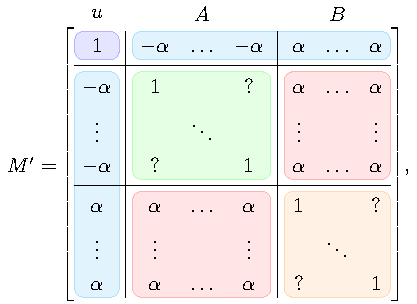
\includegraphics{images/colored-matrix}
    \end{figure}
    \vspace{-0.5em}
    \noindent
    where the $?$ entries can be either $-\alpha$ or $\alpha$.
    Now consider the vector $\bm{v}$ that assigns the value $\alpha$ to $u$, as well as $1 / |A|$ to each vertex in $A$ and $-1/|B|$ to each vertex in $B$.
    By upper bounding all the $?$ entries of $M'$ by $\alpha$, we then obtain 
    \begin{figure}[H]
        \centering
        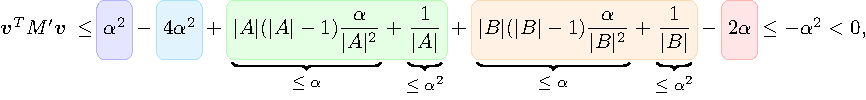
\includegraphics{images/colored-equation}
    \end{figure}
    % \begin{align*}
    %     \bm{v}^T M' \bm{v} 
    %         &\le \alpha^2 - 4\alpha^2 + \underbrace{|A|( |A| - 1) \frac{\alpha}{|A|^2}}_{\le \alpha} + \underbrace{\frac{1}{|A|}}_{\le \alpha^2} + \underbrace{|B|( |B| - 1)\frac{\alpha}{|B|^2}}_{\le \alpha} + \underbrace{\frac{1}{|B|}}_{\le \alpha^2} -\; 2 \alpha  
    %         % &\le \alpha ^2 + \frac{1}{|A|} + \frac{1}{|B|} - 4 \alpha^2 
    %         \le -\alpha^2 < 0,
    % \end{align*}
    \vspace{-0.5em}
    \noindent
    contradicting the positive semidefiniteness of $M$. 
    We conclude that such a configuration cannot exist.
\end{proof}

\begin{figure}[ht]
    \centering
    \includestandalone{tikz/forbidden-configuration}
    \captionsetup{justification=centering, margin=2cm}
    \caption{Forbidden type (ii) configuration}
    \label{fig:forbidden-typeii-config}
\end{figure}

Now we want to prove Theorem \ref{thm:bounded-degree-associated-graph}.
Recall that for a set of equiangular lines, we constructed the associated graph $G$ by choosing an arbitrary set of unit vectors that represents the equiangular set.
Replacing any of these unit vectors $\bm{u}$ by $-\bm{u}$ has the effect of exchanging the neighbours and non-neighbours of $\bm{u}$ in $G$. 
Using the forbidden induced subgraphs of the above lemma, we are going to argue that we can switch some of the vectors to obtain a bounded-degree graph.

\begin{proof}[Proof of Theorem \ref{thm:bounded-degree-associated-graph}]
    Fix $\alpha > 0$.
    Given a set of $n$ equiangular lines in $\R^d$ with pairwise angle $\arccos \alpha$, choose unit vectors $\bm{x}_1, \dots, \bm{x}_n$ along the lines arbitrarily.
    Let $G$ be the associated graph with vertex set $\{ \bm{x}_1, \dots, \bm{x}_n \}$ and an edge between $\bm{x}_i$ and $\bm{x}_j$ whenever $\langle \bm{x}_i, \bm{x}_j \rangle = -\alpha$.
    Let $M_1$, $M_2$ be defined as in Lemma \ref{lem:forbidden-induced-subgraphs}, and let $M = M_2^2 + 2M_2$.
    By Ramsey's theorem, there exists a constant $R = R(M_1, M)$ such that any graph on at least $R$ vertices contains either a clique of size $M_1$ or an independent set of size $M$.
    If $n = |G|\; < R$, we can bound $\Delta (G) \le R$ and are done. 
    (Note that $R$ only depends on $M_1$ and $M$, which in turn only depend on $\alpha$.)
    
    Hence, assume $|G|\; \ge R$. 
    Since $G$ does not contain a clique of size $M_1$ by the lemma, there must be an independent set $S \subseteq V(G)$ of size $M$.

    Consider any vertex $\bm{u} \in V(G) \setminus S$. 
    Let $V_1 = S \cap N_G(\bm{u})$ be the set of neighbours of $\bm{u}$ in $S$, and let $V_2 = S \setminus V_1$. 
    Since both $V_1$ and $V_2$ are contained in the independent set, there are no edges between $V_1$ and $V_2$. 
    By Lemma \ref{lem:forbidden-induced-subgraphs}, one of $V_1, V_2$ must contain fewer than $M_2$ vertices, since otherwise, we would have a forbidden type (ii) configuration.
    In the case where $|V_1|\; > M_2$, we replace $\bm{u}$ by $-\bm{u}$, so that $-\bm{u}$ has at most $M_2$ neighbours in $S$ in the resulting graph.
    After performing this procedure for each $\bm{u} \in V(G) \setminus S$, we may assume that every vertex in $G$ has at most $M_2$ neighbours in $S$.

    We claim that the resulting graph $G$ has maximum degree at most $M_2$.
    Suppose some vertex $\bm{u}$ has degree $d_G(\bm{u}) > M_2$. 
    Let $A \subseteq N_G(\bm{u})$ be a subset of the neighbourhood of size $M_2$. 
    Recall that $\bm{u}$ as well as each vertex in $A$ has at most $M_2$ neighbours in $S$, so 
    \begin{equation*}
        |S \cap N_G(\{ \bm{u}\} \cup A) |\; \le (M_2 + 1) M_2.
    \end{equation*}
    Define $B = S \setminus N_G(\{ \bm{u} \} \cup A)$. 
    Then there are no edges between $A$ and $B$, and 
    \begin{equation*}
        |B|\; \ge |S|\, -\, (M_2 + 1) M_2 = M_2.
    \end{equation*}
    Hence, $\bm{u}, A, B$ forms a forbidden type (ii) configuration, contradicting Lemma \ref{lem:forbidden-induced-subgraphs}.
    We conclude that $\Delta(G)$ is bounded by $M_2$, a constant depending only on $\alpha$.
\end{proof}

% \begin{lemma}
%     The largest clique in $G$ has size at most $\alpha^{-1} + 1$.
% \end{lemma}

% \begin{proof}
%     Consider a clique in $G$ consisting of unit vectors $\bm{x}_1, \dots, \bm{x}_K$, so that $\bm{x}_i ^T \bm{x}_j = -\alpha$ for $i \ne j$.
%     Then we have 
%     \begin{equation*}
%         0 \le \| \bm{x}_1 + \dots + \bm{x}_K \| ^2\; = \sum \limits_{i = 1}^K \underbrace{\bm{x}_i ^T \bm{x}_i}_{= 1} + \sum \limits_{i \ne j} \underbrace{\bm{x}_i^T \bm{x}_j}_{= -\alpha} = K - K(K - 1) \alpha.
%     \end{equation*}
%     Hence, $K \ge K(K - 1) \alpha$, so $K \le \alpha^{-1} + 1$.
% \end{proof}

% \begin{definition}
%     Let $G$ be a graph. 
%     For subsets $A \subseteq X \subseteq V(G)$, define $C_X (A)$ to be the set of vertices in $V(G) \setminus X$ that are adjacent to all vertices in $A$ and to none in $X \setminus A$.
% \end{definition}

\section{Bounding the second eigenvalue multiplicity} 
    \label{section:snd-eigval-multiplicity}
In this section, we prove Theorem \ref{thm:snd-eigval-multiplicity}, which provides the sublinear bound on the second eigenvalue multiplicity.
For any graph $G$ and $\lambda \in \R$, we denote the multiplicity of $\lambda$ as an eigenvalue of $G$ by $m_G(\lambda)$.
If $\lambda$ is not an eigenvalue, then $m_G(\lambda) = 0$.

First of all, let us discuss the necessity of the assumptions of the theorem. 
The restriction on connected graphs cannot be dropped since $\lambda_2$ can be the spectral radius of linearly many small components.  
For instance, the disjoint union of $n / 2$ edges has spectral radius $1$ with \mbox{multiplicity $n/2$}.

The example of the complete graph $K_n$ illustrates that graphs with an unbounded maximum degree need not have sublinear second eigenvalue multiplicity, as $K_n$ has second eigenvalue $-1$ with multiplicity $n - 1$.

Via a slight modification of the proof we are about to discuss, one can show that for any constant $j$, the multiplicity of the $j$-th eigenvalue is $O_{\Delta, j} (n / \log \log n)$ (see \cite{equiangular}).
However, for eigenvalues in the centre of the spectrum, the statement is false.
The following construction found in \cite{equiangularexpository}, in which each vertex of a path of length $l$ is joined with two degree-one vertices, has the eigenvalue $0$ with linear multiplicity.

\begin{figure}[H]
    \centering
    \begin{tikzpicture}
        % Define the vertices with manual positions
        \mynode (v1) at (0, 1) {};
        \mynode (v2) at (0.5, 0) {};
        \mynode (v3) at (1, 1) {};

        \mynode (v4) at (2, 1) {};
        \mynode (v5) at (2.5, 0) {};
        \mynode (v6) at (3, 1) {};

        \mynode (v7) at (4, 1) {};
        \mynode (v8) at (4.5, 0) {};
        \mynode (v9) at (5, 1) {};

        \node[circle, draw=white, fill=white, inner sep=2pt, minimum size=5pt] (x1) at (5.5, 0) {};
        \node at (6.5, 0.5) {\ldots};
        \node[circle, draw=white, fill=white, inner sep=2pt, minimum size=5pt] (x2) at (7.5, 0) {};

        \mynode (v10) at (8, 1) {};
        \mynode (v11) at (8.5, 0) {};
        \mynode (v12) at (9, 1) {};

        \node at (v1) [above = .1cm] {0};
        \node at (v3) [above = .1cm] {0};

        \node at (v4) [above = .1cm] {-1};
        \node at (v6) [above = .1cm] {1};

        \node at (v7) [above = .1cm] {0};
        \node at (v9) [above = .1cm] {0};

        \node at (v10) [above = .1cm] {0};
        \node at (v12) [above = .1cm] {0};
        
        \node at (v2) [below = .1cm] {0};
        \node at (v5) [below = .1cm] {0};
        \node at (v8) [below = .1cm] {0};
        \node at (v11) [below = .1cm] {0};

        % % Draw the edges
        \draw (v1) -- (v2);
        \draw (v3) -- (v2);
        
        \draw (v4) -- (v5);
        \draw (v6) -- (v5);

        \draw (v7) -- (v8);
        \draw (v9) -- (v8);

        \draw (v10) -- (v11);
        \draw (v12) -- (v11);

        \draw (v2) -- (v5);
        \draw (v2) -- (v8);
        \draw (x1) -- (v8);
        \draw (x2) -- (v11);
    \end{tikzpicture}
    \captionsetup{justification=centering, margin=2cm}
    \caption{One of the $0$-eigenvectors of the graph}
    \label{fig:modified-path}
\end{figure}
To see that, consider any vertex $v_i$ on the path, $i \in [l]$.
The vector assigning $1$ to one of the degree-one neighbours of $v_i$, $-1$ to the other and $0$ to all remaining vertices (see Figure \ref{fig:modified-path}) is an eigenvector for the eigenvalue $0$.
These eigenvectors are linearly independent for distinct $i$, so the eigenvalue $0$ has multiplicity at least $l$.

In order to prove the theorem, we first need a few lemmas.

\begin{lemma} \label{lem:bound-size}
    Let $G$ be a graph with $\lambda_2(G) \le 0$. 
    Then $e(G) \le \Delta(G)^2$.
\end{lemma}

\begin{proof}
    Let $n$ = $|G|$, and let $\lambda_1 \ge \dots \ge \lambda_n$ denote the eigenvalues of $G$. We have
    \begin{align*}
        2e(G) = \sum \limits_{i = 1}^n \lambda_i ^2 = \lambda_1^2 + \sum \limits_{i = 2}^n \lambda_i ^2 
        \le \lambda_1^2 + \left( \sum \limits_{i = 2}^n \lambda_i \right)^2 
        = \lambda_1^2 + (-\lambda_1)^2 \le 2 \Delta(G)^2 .
    \end{align*}
    The middle inequality holds because $\lambda_i \le 0$ for all $i \ge 2$.
\end{proof}

\begin{definition}
    An \textit{$r$-net} in $G$ is a subset $U \subseteq V(G)$ such that every vertex in $G$ is within distance $r$ from some vertex in $U$.

    The \textit{$r$-neighbourhood} of a vertex $v$ in $G$, denoted $G_r(v)$, is the subgraph of $G$ induced by all vertices that are at distance at most $r$ from $v$.
\end{definition}

At a very high level, the proof of the theorem proceeds as follows. 
First, we are going to remove a net of small size from our graph. 
We shall see that this significantly reduces the spectral radii of neighbourhoods in $G$ (i.e. the \textit{local spectral radii}), which will allow us to derive a bound on the multiplicity of the second eigenvalue in the remaining graph.
To bound the multiplicity in the original graph, we then use the following observation.

\begin{observation} \label{observation:interlacing}
    Let $G$ be a graph with eigenvalue $\lambda$. 
    Removing $k$ vertices from $G$ does not decrease the multiplicity of $\lambda$ by more than $k$.
\end{observation}

\begin{proof}
    Let $\lambda_1 \ge \dots \ge \lambda_n$ denote the eigenvalues of $G$.
    If we remove one vertex $v$ from $G$, the eigenvalues $\mu_1 \ge \dots \ge \mu_{n - 1}$ of $G - v$ interlace those of $G$:
    \begin{equation*}
        \lambda_1 \ge \mu_1 \ge \lambda_2 \ge \mu_2 \ge \dots \ge \mu_{n - 1} \ge \lambda_n.
    \end{equation*}
    Hence, if the multiplicity of $\lambda$ in $G$ is $m$, its multiplicity in $G - v$ is at least $m - 1$.
    Iterating the argument $k$ times yields the observation.
\end{proof}

The next lemma guarantees the existence of small nets.
\begin{lemma} \label{lem:small-r-net}
    Let $n, r$ be positive integers. Every connected graph $G$ on $n$ vertices has an $r$-net of size at most $\lceil \frac{n}{r + 1} \rceil$
\end{lemma}

\begin{proof}
    We can assume that $G$ is a tree, otherwise consider a spanning tree of $G$.
    We construct an $r$-net of the desired size as follows:
    Pick an arbitrary vertex $v$, and a vertex $w$ with maximum distance from $v$. 
    If $\dist_G (v, w) \le r$, then $\{ v \}$ is an $r$-net and we are done.
    Otherwise, let $u$ be the vertex on the path between $v$ and $w$ at distance $r$ from $w$. 
    We add $u$ to the net and iterate the procedure on the component of $G - u$ that \mbox{contains $v$}. 
    Since the remaining tree has at most $n - (r + 1)$ vertices, this yields an $r$-net of size at most $\lceil \frac{n}{r + 1} \rceil$.
\end{proof}

Removing a net destroys closed walks in a graph and hence reduces the spectral radius.

\begin{lemma} \label{lem:net-removal}
    Let $G$ be a graph, $r \in \N$, and let $H$ be a subgraph obtained from $G$ by deleting an $r$-net. 
    Then 
    \begin{equation*}
        \lambda_1 (H)^{2r} \le \lambda_1 (G)^{2r} - 1.
    \end{equation*}
\end{lemma}

\begin{proof}
    We can assume that $G$ has no isolated vertices because these do not affect the spectral radius.
    For each $v \in V(H)$, the number of closed walks of length $2r$ starting at $v$ is strictly less in $H$ than in $G$. 
    Indeed, in $G$ one can walk from $v$ to a vertex of the $r$-net and back (and possibly walk back and forth along a single edge to reach the length $2r$), and this walk no longer exists in $H$.
    Therefore, $A_H^{2r} \le A_G^{2r} - I$ (padding zeros to extend $A_H$ to a matrix of size $|G| \times |G|$). 
    By the Perron--Frobenius theorem, it follows that 
    \begin{equation*}
        \lambda_1 (H)^{2r} = \lambda_1 ( A_H ^{2r}) \le \lambda_1 ( A_G ^{2r} - I) = \lambda_1 (G)^{2r} - 1.
    \end{equation*}
\end{proof}

The next lemma establishes a connection between the spectrum of a graph and its local spectral radii.
\begin{lemma} \label{lem:local-radii}
    For every graph $G$ and every $r \in \N$, 
    \begin{equation*}
        \sum \limits_{i = 1}^{|G|} \lambda_i (G) ^{2r} \le \sum \limits_{v \in V(G)} \lambda_1 (G_r (v))^{2r}.
    \end{equation*}
\end{lemma}

\begin{proof}
    Recall that 
    \begin{equation*}
        \sum \limits_{i = 1}^{|G|} \lambda_i (G) ^{2r} = \tr A_G^{2r},
    \end{equation*}
    so the left-hand side counts the number of closed walks of length $2r$ in $G$.
    Consider a vertex $v \in V(G)$. 
    A closed walk of length $2r$ starting at $v$ must stay within distance $r$ from $v$, so the number of such walks in $G$ equals the number in $G_r(v)$.
    By Lemma \ref{lem:bounding-walks}, the number of closed walks of length $2r$ in $G_r(v)$ starting at $v$ is at most $\lambda_1(G_r (v))^{2r}$. 
    Hence, the right-hand side is an upper bound for the number of closed walks in $G$, and the inequality follows.
\end{proof}

Now we are ready to prove the theorem, mostly following the version of the proof in \cite{equiangularexpository}.

\begin{proof}[Proof of Theorem \ref{thm:snd-eigval-multiplicity}]
    Let $G$ be a connected graph on $n$ vertices.
    For ease of notation, let $\lambda = \lambda_2(G)$.
    We can assume that $\lambda > 0$ since otherwise $G$ has bounded size by Lemma \ref{lem:bound-size} (and hence also bounded second eigenvalue multiplicity).
    We can also assume that $\Delta \ge 2$, since otherwise $G$ consists only of a single edge.
    
    Define $r = \lfloor c \log \log n \rfloor$ and $s = \lfloor c \log n \rfloor$, where $c = c(\Delta) > 0$ is a sufficiently small constant to be determined later.

    Suppose there is a vertex $v$ with $\lambda_1 (G_{s + 1} (v)) > \lambda$.
    Then Lemma \ref{lem:disjoint-subgraphs} tells us that the spectral radius of $G \setminus G_{s + 2} (v)$ is strictly smaller than $\lambda$; in particular, $\lambda$ is not an eigenvalue of $G \setminus G_{s + 2} (v)$.  
    Recall that by Observation \ref{observation:interlacing}, the multiplicity of $\lambda$ cannot decrease by more than $|G_{s + 2} (v)|$ when removing $G_{s + 2} (v)$. 
    Thus, the multiplicity of $\lambda$ in $G$ is at most 
    \begin{equation*}
        |G_{s + 2} (v)|\; \le 1 + \Delta^{s + 2} \le 1 + \Delta^{c \log n + 2} = 1 + \Delta^2 n^{c \log \Delta} = O(\sqrt{n}),
    \end{equation*}
    if $c$ is chosen to be at most $(2 \log \Delta)^{-1}$.

    Henceforth assume $\lambda_1 (G_{s + 1} (v)) \le \lambda$ for all $v \in V(G)$.
    Let $U$ be an $r$-net of size $\lceil n / (r + 1) \rceil$ in $G$, whose existence is guaranteed by Lemma \ref{lem:small-r-net}, and let $H = G - U$. 
    We wish to bound the multiplicity of $\lambda$ in $H$.
    By Lemma \ref{lem:local-radii},
    \begin{equation*}
        m_H (\lambda) \cdot \lambda^{2s} \le \sum \limits_{i = 1}^{|H|} \lambda_i(H)^{2s} \le \sum \limits_{v \in V(H)} \lambda_1 (H_s (v))^{2s}.
    \end{equation*}

    Furthermore, for every $v \in V(H)$, the vertices in $G_{s + 1} (v) \setminus H_s (v)$ form an $r$-net of $G_{s + 1} (v)$.
    Indeed, starting from any vertex in $G_{s + 1} (v)$, we can walk to a vertex $u \in U$, making at most $r$ steps.
    If $u$ is at distance at most $s + 1$ from $v$ in $G$, we have $u \in G_{s + 1} (v) \setminus H_s (v)$ (note that $u \notin V(H)$ by the definition of $H$).
    Otherwise, the path to $u$ uses a vertex at distance exactly $s + 1$ from $v$, and that vertex is contained in $G_{s + 1} (v) \setminus H_s (v)$.

    For every $v \in V(H)$, it follows by Lemma \ref{lem:net-removal} that 
    \begin{equation*}
        \lambda_1 (H_s (v))^{2r} \le \lambda_1 (G_{s + 1}(v)) ^{2r} - 1 \le \lambda^{2r} - 1.
    \end{equation*}
    Hence,
    \begin{equation*}
        \lambda_1 (H_s (v))^{2s} \le (\lambda^{2r} - 1)^{\frac{s}{r}}.
    \end{equation*}
    Combining the inequalities, we obtain
    \begin{equation*}
        m_H (\lambda) \cdot \lambda^{2s} \le n (\lambda^{2r} - 1)^{\frac{s}{r}}.
    \end{equation*}
    Thus, using the inequality $1 + x \le e^x$, 
    \begin{align*}
        m_H (\lambda) &\le \frac{n}{\lambda^{2s}} (\lambda^{2r} - 1)^{\frac{s}{r}} 
            = n \cdot \left ( \frac{1}{\lambda^{2r}} ( \lambda^{2r} - 1) \right) ^{\frac{s}{r}} \\ 
        &= n \cdot (1 - \lambda^{-2r})^{\frac{s}{r}} 
            \le n \cdot e ^{-\frac{s}{r} \cdot \lambda^{-2r}} 
            \le n \cdot e^{-\sqrt{\log n}}.
    \end{align*}
    For the last inequality, we have used that $\lambda \le \lambda_1 \le \Delta$ and therefore,
    \begin{align*}
        \frac{s}{r} \cdot \lambda^{-2r} &\ge \frac{c \log n - 1}{c \log \log n} \cdot \Delta^{-2 c \log \log n} \\ 
        &\ge \frac{\log n}{2 \log \log n} \cdot (\log n)^{-2 c \log \Delta} = \frac{(\log n)^{1 - 2c \log \Delta}}{2 \log \log n} \ge \sqrt{\log n},
    \end{align*}
    provided that $c$ is chosen smaller than $(4 \log \Delta)^{-1}$ and $n$ is large enough.

    Finally, we apply Observation \ref{observation:interlacing}. 
    Since $H$ is obtained from $G$ by removing an $r$-net consisting of at most $\lceil n / (r + 1) \rceil$ vertices, 
    \begin{equation*}
        m_G(\lambda) \le m_H(\lambda) + \left \lceil \frac{n}{r + 1} \right \rceil \le \frac{n}{e^{\sqrt{\log n}}} + \left \lceil \frac{n}{c \log \log n} \right \rceil
            = O \Big(\frac{n}{\log \log n} \Big),
    \end{equation*}
    which completes the proof.
\end{proof}

Since no construction of a bounded-degree graph with second eigenvalue multiplicity \sloppy $\Theta(n / \log \log n)$ is known, the authors of \cite{equiangular} conjectured that the bound in Theorem \ref{thm:snd-eigval-multiplicity} can be improved.
Observe that any improvement on the size of an $r$-net immediately yields a stronger bound on the second eigenvalue multiplicity by the same proof. 
In the conclusion of the paper \cite{equiangular}, it is remarked that the existence of smaller nets can be guaranteed among expander graphs.\footnote{Here we use a slightly different notion of expansion than in Section \ref{section:cheeger}, considering neighbouring vertices instead of edge boundaries.}

% Now fix an $n$-vertex graph $G$ with maximum degree at most $\Delta$. 
% Suppose $G$ is an expander graph in the sense that $|N_G(A)|\; \ge (1 + \varepsilon) |A|$ for all $A \subseteq V(G)$ with $|A|\; \le \frac{n}{2}$ for some $\varepsilon > 0$.


\begin{lemma}
    Let $G$ be a graph of order $n$.
    Suppose there exists $\varepsilon > 0$ such that $|N_G(A)|\; \ge (1 + \varepsilon) |A|$ for all $A \subseteq V(G)$ with $|A|\; \le \frac{n}{2}$.
    Then, for every $r \in \N$, the graph $G$ contains an $r$-net of size at most \mbox{$n / (1 + \varepsilon)^{\lfloor r / 2 \rfloor}$}.
\end{lemma}

\begin{proof}
    Let $S \subseteq V(G)$ be a maximal $r$-separated set in $G$, that is, a maximal subset of the vertices in $G$ such that any two vertices in $S$ have distance at least $r + 1$.
    Then $S$ is an $r$-net in $G$: Suppose there was a vertex $v$ not within distance at most $r$ from any vertex \mbox{in $S$}. 
    Then $S \cup \{ v\}$ would form a larger $r$-separated set, contradicting the maximality \mbox{of $S$}.

    It remains to show that $|S|\; \le n / (1 + \varepsilon)^{\lfloor r / 2 \rfloor}$.
    For any vertex $v \in S$, consider its $\lfloor r /2 \rfloor$-neighbourhood $G_{\lfloor r /2 \rfloor} (v)$.
    Due to the expansion property, 
    \begin{equation*}
        |G_{\lfloor r /2 \rfloor} (v)|\; \ge (1 + \varepsilon) ^{{\lfloor r / 2 \rfloor}}.
    \end{equation*}
    By the definition of $S$, the ${\lfloor r / 2 \rfloor}$-neighbourhoods of the vertices in $S$ are necessarily disjoint.
    We conclude that $n \ge |S| \cdot (1 + \varepsilon) ^{{\lfloor r / 2 \rfloor}}$, as claimed.
\end{proof}

Now let $G$ be an expander graph as in the lemma.
Let $r = \lfloor c \log \log n \rfloor$ as in the proof of Theorem \ref{thm:snd-eigval-multiplicity},
and suppose $U$ is an $r$-net of size at most $n / (1 + \varepsilon)^{\lfloor r / 2 \rfloor}$ in $G$. 
We have 
\begin{equation*}
    (1 + \varepsilon)^{\lfloor r / 2 \rfloor} \ge (1 + \varepsilon)^{ c \log \log n} = (\log n)^{c \log (1 + \varepsilon)} \ge (\log n)^\alpha
\end{equation*}
for any $\alpha \le c \log (1 + \varepsilon)$.
Hence, $|U|\; \le n / (\log n)^\alpha$, 
and we obtain:

\begin{corollary}
    Fix $\Delta > 0$ and $\varepsilon > 0$.
    Let $G$ be an $n$-vertex graph with maximum degree at most $\Delta$, and suppose $G$ satisfies $|N_G(A)|\; \ge (1 + \varepsilon) |A|$ for all $A \subseteq V(G)$ with $|A|\; \le \frac{n}{2}$.
    Then there exists a constant $\alpha$ depending only on $\Delta$ and $\varepsilon$ such that
    \begin{equation*}
        m_G (\lambda_2) \le O_{\Delta} \left(\frac{n}{(\log n)^\alpha} \right).
    \end{equation*}
\end{corollary}

\begin{remark}
    The authors of \cite{equiangular} even claim that for an expander graph as in the corollary, the second eigenvalue multiplicity is at most $O_{\Delta, \varepsilon}(n / \log n)$. 
    However, this does not follow directly from their proof, so we think that it is an inaccuracy.
\end{remark}

It remains an intriguing problem to determine the optimal bounds for general graphs in Theorem \ref{thm:snd-eigval-multiplicity}.
The currently best-known lower bound comes from a family of graphs with maximum degree $4$ and second eigenvalue multiplicity at least $\sqrt{n / \log_2 n}$ \mbox{(see \cite{snd-eigval-lower-construction}).}
Therefore, the following question suggests itself:
\begin{question}
    Does there exist a constant $\alpha > 0$, such that every $n$-vertex connected graph with maximum degree at most $\Delta$ has second eigenvalue multiplicity at most \mbox{$O_\Delta (n^{1 - \alpha})$}?
\end{question}
Despite the relatively large gap between the lower bound constructions and the upper bounds, and even though the paper of Jiang et al. \cite{equiangular} appears to have initiated some research in that direction, no significantly stronger result has been found for general graphs yet.
However, McKenzie, Rasmussen, and Srivastava \cite{mckenzie2023supportclosedwalkssecond} established the following improved bound for regular graphs.
\begin{theorem}[\cite{mckenzie2023supportclosedwalkssecond}, Theorem 4.1]
    Let $d \in \N$. Every $d$-regular graph $G$ on $n$ vertices satisfies
    \begin{equation*}
        m_G (\lambda_2) = O_d \bigg( \frac{n \log \log n }{\log ^{1/5} n}\bigg).
    \end{equation*}
\end{theorem}

On a high level, their proof strategy is similar to that from \cite{equiangular} for Theorem \ref{thm:snd-eigval-multiplicity}. 
The main difference is that in \cite{mckenzie2023supportclosedwalkssecond}, they analysed random walks in regular graphs and showed that a typical random walk uses a "large" number of vertices. 
They concluded that by removing a small set of vertices chosen randomly, many of these walks are destroyed, which they could in turn use to derive a bound on the second eigenvalue multiplicity of the remaining graph.
The improvement comes from the fact that they were able to delete only $O (n \log \log n / \log ^{1/5} n)$ vertices, as opposed to $O(n / \log \log n)$ vertices in \cite{equiangular}.

The technique used in \cite{equiangular} and \cite{mckenzie2023supportclosedwalkssecond} to estimate $m_G(\lambda_2)$ is also known as the \textit{trace method} or \textit{moment method}. 
In general, one starts by estimating the number of closed walks of length $2k$ in a graph $G$. 
Recall that this number is equal to 
\begin{equation*}
    \tr A_G^{2k} = \sum_{i = 1}^{|G|} \lambda_i^{2k}.
\end{equation*}
Now one relies on the idea that for large $k$, the sum on the right-hand side will be dominated by $\lambda_1^{2k} + m_G(\lambda_2) \cdot \lambda_2^{2k}$, which can be used to bound $\lambda_2$ or $m_G (\lambda_2)$.

Naturally, these estimates allow for some margin of error. 
Specifically, Haiman, Schildkraut, Zhang, and Zhao \cite{snd-eigval-lower-construction} demonstrated that the proof of Theorem \ref{thm:snd-eigval-multiplicity} can be slightly modified to show that there are at most $O(n / \log \log n)$ eigenvalues within the interval $[(1 - 1/\log n) \lambda_2, \lambda_2]$.
Furthermore, they constructed a family of connected bounded-degree graphs matching this bound up to a constant factor. 
This can be seen as an indication that substantially stronger techniques may be necessary to push the upper bounds for general graphs further.

\section{Separable graphs}
Since the currently known upper bounds on the second eigenvalue multiplicity of general graphs do not appear optimal yet, it is also of interest to consider special classes of graphs. 
In this section, we show stronger bounds than in Theorem \ref{thm:snd-eigval-multiplicity} for so-called \textit{separable graphs}.
The key concept that we shall need is the following.

\begin{definition}
    Let $G$ be a graph on $n$ vertices. 
    A subset $S \subseteq V(G)$ is a \textit{(balanced) separator} if there exists a partition $V(G) \setminus  S =  A \cup B$ such that $|A|, |B|\;\le \frac{2n}{3}$ and $G$ has no edges between $A$ and $B$.
\end{definition}

A planar graph is a graph that can be drawn in the plane in such a way that no two edges intersect (for a formal definition, refer to \cite[Chapter 4]{diestel}). 
The famous planar separator theorem due to Lipton and Tarjan \cite{liptontarjan} states that every planar graph on $n$ vertices has a separator of size at most $O(\sqrt{n})$. 
This result is optimal up to constant factors, as demonstrated by the $n \times n$ grid graph (cf. Figure \ref{fig:separator-grid}).

\begin{figure}[ht]
    \centering
    \begin{tikzpicture}
        \draw[fill=green!10, draw=green!30, rounded corners] (0.5, 0.5) rectangle (1.9, 4.3);
        \draw[fill=blue!10, draw=blue!30, rounded corners] (2.1, 0.5) rectangle (2.7, 4.3);
        \draw[fill=red!10, draw=red!30, rounded corners] (2.9, 0.5) rectangle (4.3, 4.3);

        \foreach \i in {1, 2, 3, 4, 5} {
            \foreach \j in {1, 2, 3, 4, 5} { 
                \mynode (v\i\j) at (0.8 * \i, 0.8 * \j) {};
            }
        }

        \foreach \x in {1,2,3,4,5} {
            \foreach \y in {1,2,3,4,5} {
                \ifnum\x<5
                    \draw (v\x\y) -- (v\the\numexpr\x+1\relax\y);
                \fi
                \ifnum\y<5
                    \draw (v\x\y) -- (v\x\the\numexpr\y+1\relax);
                \fi
            }
        }

        % Label the rectangles
        \node at (1.2,0) {$A$};
        \node at (2.4,0) {$S$};
        \node at (3.6,0) {$B$};
    \end{tikzpicture}
    \captionsetup{justification=centering, margin=2cm}
    \caption{A balanced separator of the $5 \times 5$ grid}
    \label{fig:separator-grid}
\end{figure}

Motivated by the planar separator theorem, we consider general classes of graphs with "small" separators and bound the second eigenvalue multiplicity of such graphs.

\begin{definition}
    Let $\mathcal{G}$ be a hereditary class of graphs (that is, closed under taking induced subgraphs), 
    and let $f : \N \rightarrow \R^+$ be a function.
    We say that the graphs in $\mathcal{G}$ are \textit{$f$-separable} if any graph $G \in \mathcal{G}$ has a balanced separator of size $O(f(|G|))$.
\end{definition}

\begin{theorem} \label{thm:separable-snd-eigval-mult}
    Let $\Delta \in \N$ and $f : \N \rightarrow \R^+$ be an increasing function satisfying \mbox{$f(\frac{2}{3}n) \le \alpha f(n)$} for some $\alpha < 1$ and all $n \in \N$.
    Let $\mathcal G$ be a hereditary class of $f$-separable graphs with maximum degree at most $\Delta$. 
    Then all connected graphs in $\mathcal G$ have second eigenvalue multiplicity at most $O_{\Delta}(f)$.
\end{theorem}

\begin{proof}
    By the theorem's hypothesis, there exists a constant $R$ such that any $n$-vertex graph in $\mathcal{G}$ has a separator of size at most $R f(n)$.
    
    Let $G \in \mathcal G$ be a graph with $n$ vertices.
    As usual, we denote the eigenvalues of $G$ by $\lambda_1 \ge \dots \ge \lambda_n$.
    We use induction on $n$ to show that 
    \begin{equation*}
        m_G (\lambda_2) \le \frac{R(\Delta + 1)}{1 - \alpha} f(n).
    \end{equation*}    
    The bound trivially holds for $n = 2$.
    %\footnotemark
    (Note that we must have $Rf(2) \ge 1$.)%, as a separator cannot be empty in a connected graph.)
    %\footnotetext{Note that a separator cannot be empty in a connected graph, so we must have $Rf(2) \ge 1$.}
    
    Now let $n$ be fixed and suppose the theorem holds for all graphs with fewer than $n$ vertices. 
    Let $S \subseteq V(G)$ be a separator in $G$ of size $k\, \le R f(n)$ and define $G' = G - S$.
    If $m_G (\lambda_2) \le (\Delta + 1)k$, we are done. 
    Hence assume $m_G (\lambda_2) = m + k$ for some $m \ge \Delta k + 1$.
    % By Observation \ref{observation:interlacing}, the multiplicity of $\lambda_2$ in $G'$ is at least $m$.
    Let $\mu_1 \ge \dots \ge \mu_{n - k}$ denote the eigenvalues of $G'$.
    By the Cauchy interlacing theorem, we have 
    \begin{equation*}
        \lambda_i \ge \mu_i \ge \lambda_{i + k}, \ \ i \in [n - k].
    \end{equation*}
    In particular, as $\lambda_2 = \dots = \lambda_{m + k + 1}$,
    \begin{equation*}
        \lambda_2 = \mu_2 = \dots = \mu_{m + 1},
    \end{equation*}
    so the multiplicity of $\lambda_2$ in $G'$ is at least $m$, and $G'$ has at most one eigenvalue larger \mbox{than $\lambda_2$}.
    
    Since $G'$ has at most $\Delta k < m$ components, there is one, $C$ say, in which the eigenvalue $\lambda_2$ occurs more than once.
    By the Perron--Frobenius theorem, $\lambda_2$ cannot be the largest eigenvalue \mbox{of $C$}. 
    It follows that $\lambda_2$ is the second-largest eigenvalue of $C$.
    Moreover, by Lemma \ref{lem:disjoint-subgraphs}, no other component of $G'$ has $\lambda_2$ as an eigenvalue.
    Generously bounding $k \le (\Delta + 1)k$, we conclude that
    \begin{equation*}
        m_G(\lambda_2) \le k + m_C(\lambda_2) \le (\Delta + 1) k + m_C (\lambda_2).
    \end{equation*}
    Recall that $|C|\, \le \frac{2}{3}n$. 
    By the induction hypothesis, the latter summand is at most 
    \begin{equation*}
         \frac{R(\Delta + 1)}{1 - \alpha} f \Big( \frac{2}{3}n \Big).
    \end{equation*}
    Thus we obtain 
    \begin{align*}
        m_G( \lambda_2 ) &\le (\Delta + 1)k + \frac{R(\Delta + 1)}{1 - \alpha} f \Big( \frac{2}{3}n \Big) \\ 
        &\le R(\Delta + 1) f(n) + \frac{\alpha R (\Delta + 1)}{1 - \alpha} f(n) = \frac{R (\Delta + 1)}{1 - \alpha} f(n),
    \end{align*}
    as desired.
\end{proof}

\begin{remark}
    By the planar separator theorem, the above result provides a bound of $O_\Delta (\sqrt{n})$ for the second eigenvalue multiplicity of a connected planar graph on $n$ vertices.
    Interestingly, this is still far from the truth: In \cite{planarmultiplicty} it was shown that for such a graph, $m_G(\lambda_2) \le \Delta(G)$.
\end{remark}

To exhibit specific graph classes for which Theorem \ref{thm:separable-snd-eigval-mult} asymptotically improves existing results, we cite the following result by Alon, Seymour, and Thomas, which extends the planar separator theorem to graphs with a fixed forbidden minor.
\begin{theorem}[{\cite[(1.3)]{separatortheoremfornonplanargraphs}}]
    Let $H$ be an arbitrary graph on $h$ vertices. 
    Every $n$-vertex graph $G$ without an $H$-minor has a separator of size at most $h^{\frac{3}{2}} n^{\frac{1}{2}}$.
\end{theorem}

Using Theorem \ref{thm:separable-snd-eigval-mult} we deduce:
\begin{corollary}
    Let $\Delta \in \N$, and let $H$ be a fixed graph on $h$ vertices. 
    Let $\mathcal G$ be a family of connected graphs with maximum degree at most $\Delta$ that do not contain $H$ as a minor. 
    Then the second eigenvalue multiplicity of any graph $G \in \mathcal G$ on $n$ vertices is at most $O_{\Delta, h}(\sqrt{n})$.
\end{corollary}

The last proposition of this chapter states that expander graphs do not have small separators.
This implies that any graph for which Theorem \ref{thm:separable-snd-eigval-mult} yields an improvement over Theorem \ref{thm:snd-eigval-multiplicity} must be sufficiently non-expanding.

\begin{proposition}
    Let $G$ be an $n$-vertex graph, and suppose $G$ satisfies $N_G(A) \ge (1 + \varepsilon) |A|$ for all $A \subseteq V(G)$ with $|A|\; \le n/2$ for some $\varepsilon > 0$.
    Let $S$ be a balanced separator in $G$. 
    Then 
    \begin{equation*}
        |S| \; \ge \frac{\varepsilon n}{3(1 + \varepsilon )}.
    \end{equation*}
\end{proposition}

\begin{proof}
    Consider a partition $A \cup B$ of $V(G) \setminus S$ such that $|A|, |B|\; \le 2n/3$ \mbox{and $e(A, B) = 0$}.
    We can assume that $|A|\; \le |B|$, so in particular $|A|\; \le n/2$.
    Then $|A|\, +\, |S|\; \ge n/3$.
    Clearly, we have $N_G(A) \setminus A \subseteq S$. 
    Hence, 
    \begin{equation*}
        |S|\; \ge |N_G(A) \setminus A|\; \ge \varepsilon |A|.
    \end{equation*}
    It follows that 
    \begin{equation*}
        \frac{n}{3} \le |S| + |A|\; \le (1 + \varepsilon^{-1}) |S|,
    \end{equation*}
    and the claimed inequality is obtained by solving for $|S|$.
\end{proof}

More about the connection between expanders and separators can be found in the survey \cite{krivelevich}.